% =============================================================================
% Drone GCS — Technical Code Documentation
% PAE-EDISA 2025-2026 · UPC
% =============================================================================
\documentclass[11pt,a4paper]{article}

% ── Packages ─────────────────────────────────────────────────────────────────
\usepackage[utf8]{inputenc}
\usepackage[T1]{fontenc}
\usepackage[english]{babel}
\usepackage[margin=2.4cm]{geometry}
\usepackage{lmodern}
\usepackage{microtype}
\usepackage{hyperref}
\usepackage{xcolor}
\usepackage{listings}
\usepackage{booktabs}
\usepackage{longtable}
\usepackage{array}
\usepackage{enumitem}
\usepackage{graphicx}
\usepackage{tikz}
\usetikzlibrary{shapes.geometric, arrows.meta, positioning, fit, backgrounds}
\usepackage{tcolorbox}
\tcbuselibrary{skins, breakable}
\usepackage{fancyhdr}
\usepackage{titlesec}
\usepackage{parskip}
\usepackage{amsmath}

% ── Colours ──────────────────────────────────────────────────────────────────
\definecolor{navyblue}{HTML}{1B3D6F}
\definecolor{cyanaccent}{HTML}{4FC3F7}
\definecolor{darkbg}{HTML}{0D1B2A}
\definecolor{codebg}{HTML}{F4F6F8}
\definecolor{codenumber}{HTML}{888888}
\definecolor{keywordcolor}{HTML}{1B3D6F}
\definecolor{stringcolor}{HTML}{2E7D32}
\definecolor{commentcolor}{HTML}{757575}
\definecolor{notebg}{HTML}{E3F2FD}
\definecolor{noteborder}{HTML}{4FC3F7}
\definecolor{warnbg}{HTML}{FFF8E1}
\definecolor{warnborder}{HTML}{FFA726}

% ── Hyperlinks ────────────────────────────────────────────────────────────────
\hypersetup{
  colorlinks=true,
  linkcolor=navyblue,
  urlcolor=cyanaccent,
  citecolor=navyblue,
  pdftitle={Drone GCS — Technical Code Documentation},
  pdfauthor={PAE-EDISA 2025-2026},
}

% ── Section heading style ─────────────────────────────────────────────────────
\titleformat{\section}
  {\large\bfseries\color{navyblue}}
  {\thesection.}{0.6em}{}
  [\vspace{-0.3em}\textcolor{cyanaccent}{\rule{\linewidth}{1.5pt}}]

\titleformat{\subsection}
  {\normalsize\bfseries\color{navyblue}}
  {\thesubsection.}{0.5em}{}

\titleformat{\subsubsection}
  {\normalsize\bfseries\color{darkbg}}
  {\thesubsubsection.}{0.4em}{}

% ── Code listings ─────────────────────────────────────────────────────────────
\lstdefinestyle{python}{
  language=Python,
  backgroundcolor=\color{codebg},
  basicstyle=\ttfamily\footnotesize,
  keywordstyle=\bfseries\color{keywordcolor},
  stringstyle=\color{stringcolor},
  commentstyle=\itshape\color{commentcolor},
  numberstyle=\tiny\color{codenumber},
  numbers=left,
  numbersep=8pt,
  frame=single,
  framerule=0.4pt,
  rulecolor=\color{navyblue!30},
  breaklines=true,
  showstringspaces=false,
  tabsize=4,
  captionpos=b,
  belowcaptionskip=4pt,
}

\lstdefinelanguage{JavaScript}{
  keywords={break,case,catch,class,const,continue,debugger,default,delete,do,
             else,export,extends,finally,for,function,if,import,in,instanceof,
             let,new,return,static,super,switch,this,throw,try,typeof,var,void,
             while,with,yield,async,await,of},
  sensitive=true,
  comment=[l]{//},
  morecomment=[s]{/*}{*/},
  morestring=[b]',
  morestring=[b]",
  morestring=[b]`,
}
\lstdefinestyle{javascript}{
  language=JavaScript,
  backgroundcolor=\color{codebg},
  basicstyle=\ttfamily\footnotesize,
  keywordstyle=\bfseries\color{keywordcolor},
  stringstyle=\color{stringcolor},
  commentstyle=\itshape\color{commentcolor},
  numberstyle=\tiny\color{codenumber},
  numbers=left,
  numbersep=8pt,
  frame=single,
  framerule=0.4pt,
  rulecolor=\color{navyblue!30},
  breaklines=true,
  showstringspaces=false,
  tabsize=2,
  captionpos=b,
}

\lstdefinestyle{bash}{
  language=bash,
  backgroundcolor=\color{codebg},
  basicstyle=\ttfamily\footnotesize,
  keywordstyle=\bfseries\color{keywordcolor},
  commentstyle=\itshape\color{commentcolor},
  numberstyle=\tiny\color{codenumber},
  numbers=left,
  numbersep=8pt,
  frame=single,
  framerule=0.4pt,
  rulecolor=\color{navyblue!30},
  breaklines=true,
  showstringspaces=false,
  captionpos=b,
}

% ── Note / Warning boxes ─────────────────────────────────────────────────────
\newtcolorbox{notebox}{
  colback=notebg, colframe=noteborder,
  leftrule=4pt, toprule=0.4pt, bottomrule=0.4pt, rightrule=0.4pt,
  boxsep=2pt, left=6pt, right=6pt, top=4pt, bottom=4pt,
  breakable
}

\newtcolorbox{warnbox}{
  colback=warnbg, colframe=warnborder,
  leftrule=4pt, toprule=0.4pt, bottomrule=0.4pt, rightrule=0.4pt,
  boxsep=2pt, left=6pt, right=6pt, top=4pt, bottom=4pt,
  breakable
}

% ── File-header box ───────────────────────────────────────────────────────────
\newtcolorbox{filebox}[1]{
  colback=navyblue!8, colframe=navyblue,
  title={\textbf{\texttt{#1}}},
  fonttitle=\small\color{white},
  coltitle=white, attach boxed title to top left,
  boxed title style={colback=navyblue, colframe=navyblue},
  breakable, top=4pt, left=6pt, right=6pt, bottom=4pt,
}

% ── Header / Footer ───────────────────────────────────────────────────────────
\pagestyle{fancy}
\fancyhf{}
\fancyhead[L]{\small\color{navyblue}\textbf{Drone GCS} — Technical Documentation}
\fancyhead[R]{\small\color{navyblue}PAE-EDISA 2025--2026}
\fancyfoot[C]{\small\thepage}
\renewcommand{\headrulewidth}{0.4pt}
\renewcommand{\headrule}{\hbox to\headwidth{\color{cyanaccent}\leaders\hrule height \headrulewidth\hfill}}

% ── TikZ styles ───────────────────────────────────────────────────────────────
\tikzset{
  block/.style={rectangle, draw=navyblue, fill=navyblue!10,
                text width=3.2cm, align=center, minimum height=0.9cm,
                rounded corners=2pt, font=\small},
  gcsblock/.style={block, fill=cyanaccent!20, draw=cyanaccent!70!navyblue},
  arrow/.style={-{Stealth[length=5pt]}, thick, color=navyblue!70},
  label/.style={font=\scriptsize\itshape, color=navyblue!70},
}

% =============================================================================
\begin{document}
% =============================================================================

% ── Title page ───────────────────────────────────────────────────────────────
\begin{titlepage}
  \pagecolor{darkbg}
  \color{white}
  \vspace*{4cm}
  \begin{center}
    {\fontsize{36}{44}\selectfont\bfseries DRONE GCS}\\[0.5em]
    {\Large\color{cyanaccent} Technical Code Documentation}\\[2em]
    \textcolor{cyanaccent}{\rule{10cm}{1.5pt}}\\[2em]
    {\large Autonomous Ground Control Station for UAV Inventory Operations}\\[3em]
    \begin{tabular}{rl}
      \textbf{Project:} & PAE-EDISA 2025--2026 \\[0.3em]
      \textbf{University:} & Universitat Politècnica de Catalunya (UPC) \\[0.3em]
      \textbf{Platform:} & Raspberry Pi 5 · ROS2 Jazzy · Electron \\[0.3em]
      \textbf{Version:} & 1.0 \\
    \end{tabular}
  \end{center}
  \vfill
  \textcolor{navyblue!60}{\rule{\textwidth}{0.4pt}}\\[0.3em]
  {\small\color{gray} This document describes the internal architecture and
   code-level behaviour of every module in the Drone GCS system.
   It is intended for developers and system integrators.}
\end{titlepage}
\nopagecolor
\color{black}

\tableofcontents
\clearpage

% =============================================================================
\section{System Overview}
% =============================================================================

Drone GCS is a full-stack UAV ground control system. The software runs across
two physically distinct machines:

\begin{itemize}
  \item \textbf{Raspberry Pi 5 (onboard)} — ROS2 Jazzy node graph. Handles
        sensor data acquisition, SLAM processing, barcode detection, MAVLink
        communication with the flight controller, and the autonomous mission
        planner. Exposes the entire ROS2 topic graph over a WebSocket server
        (rosbridge) on port 9090.
  \item \textbf{GCS Laptop (ground)} — Electron desktop application. Connects
        to the Pi over Wi-Fi via rosbridge and visualises all telemetry,
        camera streams, and SLAM data in real time. No ROS installation is
        required on the laptop.
\end{itemize}

\subsection{Architecture Diagram}

\begin{center}
\resizebox{\textwidth}{!}{%
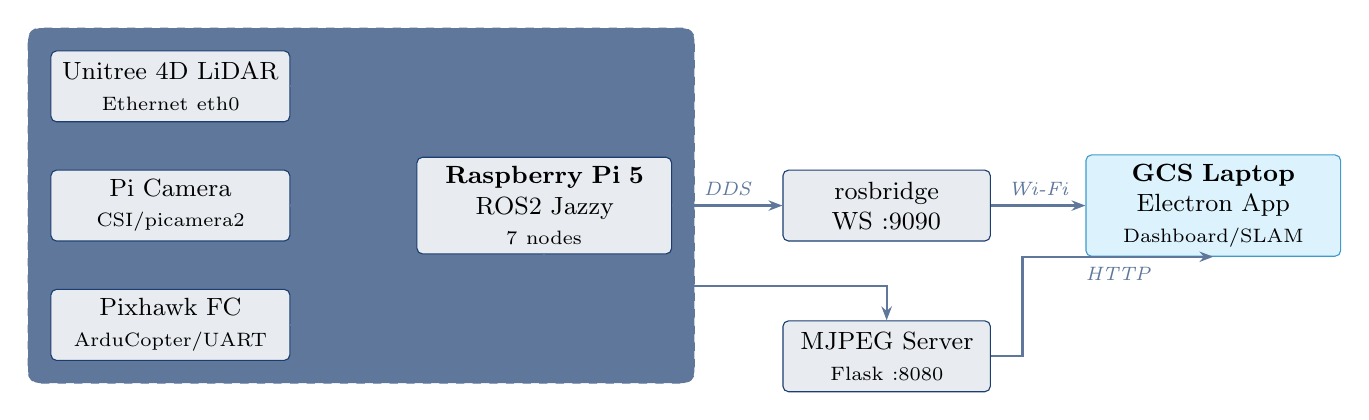
\begin{tikzpicture}[node distance=0.6cm and 1.2cm]

  % Sensor column (left)
  \node[block, text width=2.8cm] (lidar) {Unitree 4D LiDAR\\{\scriptsize Ethernet eth0}};
  \node[block, text width=2.8cm, below=of lidar] (cam) {Pi Camera\\{\scriptsize CSI/picamera2}};
  \node[block, text width=2.8cm, below=of cam]   (px)  {Pixhawk FC\\{\scriptsize ArduCopter/UART}};

  % Pi
  \node[block, text width=3.0cm, right=1.6cm of cam] (pi)
    {\textbf{Raspberry Pi 5}\\ROS2 Jazzy\\{\scriptsize 7 nodes}};

  % Arrows: sensors -> Pi
  \draw[arrow] (lidar.east) -- ++(0.6,0) |- (pi.north west) node[midway, above, label]{eth0};
  \draw[arrow] (cam.east)   -- (pi.west) node[midway, above, label]{CSI};
  \draw[arrow] (px.east)    -- ++(0.6,0) |- (pi.south west) node[midway, below, label]{UART};

  % rosbridge
  \node[block, text width=2.4cm, right=1.4cm of pi] (rb)
    {rosbridge\\WS :9090};
  \draw[arrow] (pi) -- node[above, label]{DDS} (rb);

  % GCS laptop
  \node[gcsblock, text width=3.0cm, right=1.2cm of rb] (gcs)
    {\textbf{GCS Laptop}\\Electron App\\{\scriptsize Dashboard/SLAM}};
  \draw[arrow] (rb) -- node[above, label]{Wi-Fi} (gcs);

  % MJPEG below
  \node[block, text width=2.4cm, below=1.0cm of rb] (mjpeg)
    {MJPEG Server\\{\scriptsize Flask :8080}};
  \draw[arrow] (pi.south) -- ++(0,-0.4) -| (mjpeg.north);
  \draw[arrow] (mjpeg.east) -- ++(0.4,0) |- (gcs.south) node[near end, below, label]{HTTP};

  % Drone background box
  \begin{scope}[on background layer]
    \node[draw=navyblue!30, dashed, fill=navyblue!3, rounded corners,
          fit=(lidar)(px)(pi), inner sep=8pt,
          label=above:{\small\color{navyblue}\textbf{Drone}}] {};
  \end{scope}

\end{tikzpicture}%
}
\end{center}

\subsection{Communication Protocols}

\begin{center}
\begin{tabular}{lllp{5.5cm}}
  \toprule
  \textbf{Protocol} & \textbf{Transport} & \textbf{Port} & \textbf{Purpose} \\
  \midrule
  rosbridge WebSocket & TCP / Wi-Fi & 9090 & Full ROS2 topic pub/sub from laptop \\
  MAVLink v2 & Serial UART & 57600 baud & Flight controller telemetry and commands \\
  MJPEG HTTP & TCP / Wi-Fi & 8080 & Dashboard live camera stream \\
  ROS2 DDS (RTPS) & UDP / LAN & dynamic & Inter-node communication on the Pi \\
  \bottomrule
\end{tabular}
\end{center}

% =============================================================================
\section{Raspberry Pi Stack}
% =============================================================================

All Python files are deployed to \texttt{\textasciitilde/} on the Pi and
launched by \texttt{gcs\_control.py}. The startup chain is:

\begin{center}
\texttt{rosbridge.service} $\to$ \texttt{rosbridge\_boot.sh} $\to$
\texttt{gcs\_control.py} $\to$ \emph{(dashboard buttons)} $\to$ individual nodes
\end{center}

% ---------------------------------------------------------------------------
\subsection{\texttt{rosbridge.service} \& \texttt{rosbridge\_boot.sh}}
% ---------------------------------------------------------------------------

\begin{filebox}{rosbridge.service + rosbridge\_boot.sh}
\textbf{Role:} systemd service that auto-starts on every boot.
Launches the rosbridge WebSocket server and then exec's into \texttt{gcs\_control.py}.
\end{filebox}

\subsubsection{Boot sequence}

\begin{lstlisting}[style=bash, caption=rosbridge\_boot.sh -- startup sequence]
# 1. Source the ROS2 environment (Jazzy distro)
source /opt/ros/${ROS_DISTRO:-jazzy}/setup.bash
source "$HOME/rosbridge_ws/install/setup.bash" 2>/dev/null || true
source "$HOME/slam_ws/install/setup.bash"      2>/dev/null || true

# 2. Launch rosbridge WebSocket server in the background
ros2 launch rosbridge_server rosbridge_websocket_launch.xml &
BRIDGE_PID=$!

# 3. Give rosbridge 3 s to bind port 9090 before the control node
#    tries to publish its first status message
sleep 3

# 4. Replace this shell process with gcs_control.py (exec -> no subprocess overhead)
exec python3 "$SCRIPT_DIR/gcs_control.py"
\end{lstlisting}

The \texttt{exec} on the last line is significant: the bash process is replaced
by Python, so systemd tracks the correct PID for process supervision.

The \texttt{rosbridge.service} unit sets:
\begin{itemize}
  \item \texttt{User=raspi5} — runs as the non-root user
  \item \texttt{Restart=on-failure} with \texttt{RestartSec=10} — auto-recovers from crashes
  \item \texttt{After=network-online.target} — waits for Wi-Fi before binding port 9090
  \item \texttt{Environment="ROS\_DISTRO=jazzy"} — makes the distro available inside the script
\end{itemize}

% ---------------------------------------------------------------------------
\subsection{\texttt{gcs\_control.py} — Service Manager Node}
% ---------------------------------------------------------------------------

\begin{filebox}{gcs\_control.py}
\textbf{Role:} ROS2 node that acts as a process manager for all other nodes.
Started automatically at boot alongside rosbridge.
Receives start/stop commands from the GCS dashboard and manages subprocess
lifecycle with clean process-group termination.
\end{filebox}

\subsubsection{Design}

\texttt{gcs\_control.py} is intentionally kept simple and minimal. It does not
implement any flight logic — its only job is to translate dashboard button
clicks (received as JSON on \texttt{/gcs/cmd}) into \texttt{subprocess.Popen}
calls, and to report running status back at 1 Hz on \texttt{/gcs/status}.

\begin{lstlisting}[style=python, caption=Service command table in gcs\_control.py]
SERVICE_CMDS = {
    'slam':    ['bash', f'{SCRIPTS}/slam_launch.sh'],
    'camera':  ['python3', f'{SCRIPTS}/camera_publisher.py',
                '--ros-args', '-p', 'device:=0', ...],
    'mjpeg':   ['python3', f'{SCRIPTS}/mjpeg_server.py', '0', '8080', '640', '480', '80'],
    'mavros':  ['python3', f'{SCRIPTS}/mavlink_bridge.py'],
    'brain':   ['python3', f'{SCRIPTS}/brain_node.py'],
    'barcode': ['python3', f'{SCRIPTS}/barcode_detector.py'],
}
\end{lstlisting}

\subsubsection{Process lifecycle}

Each service is started with \texttt{preexec\_fn=os.setsid} which places the
child process in its own process group. When a stop command arrives,
\texttt{os.killpg()} sends \texttt{SIGTERM} to the entire group, ensuring that
any grandchild processes (e.g. \texttt{slam\_launch.sh} and its children) are
also terminated cleanly.

\begin{lstlisting}[style=python, caption=Clean process-group termination]
def _stop(self, svc: str):
    proc = self._procs.get(svc)
    try:
        os.killpg(os.getpgid(proc.pid), signal.SIGTERM)  # kills the whole group
        proc.wait(timeout=5)
    except subprocess.TimeoutExpired:
        os.killpg(os.getpgid(proc.pid), signal.SIGKILL)  # force if still alive
\end{lstlisting}

\subsubsection{Topics}

\begin{center}
\begin{tabular}{llp{6cm}}
  \toprule
  \textbf{Topic} & \textbf{Direction} & \textbf{Payload} \\
  \midrule
  \texttt{/gcs/cmd}    & Subscribe & \texttt{\{"action":"start"|"stop","service":"slam"|...\}} \\
  \texttt{/gcs/status} & Publish @ 1 Hz & \texttt{\{"slam":"running","camera":"stopped",...\}} \\
  \bottomrule
\end{tabular}
\end{center}

% ---------------------------------------------------------------------------
\subsection{\texttt{camera\_publisher.py} — Pi Camera ROS2 Node}
% ---------------------------------------------------------------------------

\begin{filebox}{camera\_publisher.py}
\textbf{Role:} Captures frames from the Raspberry Pi Camera Module using
\texttt{picamera2} and publishes them as \texttt{sensor\_msgs/CompressedImage}
on a ROS2 topic. Consumed by \texttt{barcode\_detector.py}.
\end{filebox}

\subsubsection{Capture pipeline}

\begin{lstlisting}[style=python, caption=Camera capture and publish loop]
def _publish(self):
    # Capture a raw frame directly as a numpy array (BGR888 format)
    frame = self.cam.capture_array()
    # Encode to JPEG in-memory (no disk I/O)
    ret, buf = cv2.imencode('.jpg', frame, self._encode_params)
    if not ret:
        return
    msg = CompressedImage()
    msg.header.stamp    = self.get_clock().now().to_msg()
    msg.header.frame_id = self.fid
    msg.format          = 'jpeg'
    msg.data            = buf.tobytes()
    self.pub.publish(msg)
\end{lstlisting}

\subsubsection{QoS profile}

The publisher uses \texttt{BEST\_EFFORT / VOLATILE / KEEP\_LAST(1)}.
This is critical: any subscriber to this topic (including
\texttt{barcode\_detector.py}) must use the exact same QoS profile or it will
receive no messages — ROS2 DDS enforces QoS compatibility at subscription time.

\begin{notebox}
\textbf{Why BEST\_EFFORT?} Camera frames are time-sensitive. A reliable
(TCP-like) QoS would cause head-of-line blocking if one frame is lost, which
would freeze the stream. With BEST\_EFFORT, dropped frames are skipped
silently and the stream continues in real time.
\end{notebox}

% ---------------------------------------------------------------------------
\subsection{\texttt{mjpeg\_server.py} — Dashboard Camera HTTP Server}
% ---------------------------------------------------------------------------

\begin{filebox}{mjpeg\_server.py}
\textbf{Role:} Serves a Motion-JPEG (MJPEG) stream over HTTP on
\texttt{:8080/cam1}. Used by the Dashboard tab \texttt{<img>} element —
no ROS decoding needed on the laptop.
\end{filebox}

\subsubsection{Why two camera systems?}

The system uses two separate camera paths:

\begin{center}
\begin{tabular}{lll}
  \toprule
  \textbf{Path} & \textbf{Technology} & \textbf{Consumer} \\
  \midrule
  ROS topic & picamera2 → \texttt{CompressedImage} & barcode\_detector, icam1 \\
  MJPEG HTTP & cv2.VideoCapture (V4L2) → Flask & Dashboard cam1 \\
  \bottomrule
\end{tabular}
\end{center}

The MJPEG path is simpler and lower-latency for display. The ROS path provides
timestamped, synchronised frames for computer vision processing.

\subsubsection{Colour correction}

V4L2 on the Raspberry Pi Camera returns pixel data in RGB byte order, but
OpenCV's \texttt{imencode} expects BGR. A colour swap is applied before
encoding:

\begin{lstlisting}[style=python, caption=V4L2 colour order fix in mjpeg\_server.py]
ret, frame = cap.read()
# V4L2 on RPi Camera returns RGB-ordered data despite cv2 expecting BGR
frame = cv2.cvtColor(frame, cv2.COLOR_BGR2RGB)
_, buf = cv2.imencode('.jpg', frame, encode_params)
\end{lstlisting}

% ---------------------------------------------------------------------------
\subsection{\texttt{barcode\_detector.py} — Vision and Inventory Node}
% ---------------------------------------------------------------------------

\begin{filebox}{barcode\_detector.py}
\textbf{Role:} Subscribes to the Pi Camera ROS topic, runs barcode and QR code
detection on every frame using \texttt{pyzbar}, tags each detection with the
current SLAM position, and publishes annotated images and detection events.
\end{filebox}

\subsubsection{Processing pipeline}

\begin{center}
\begin{tikzpicture}[node distance=0.5cm and 1.2cm, every node/.style={font=\small}]
  \node[block] (cam)   {ROS Image\\\texttt{/camera/.../compressed}};
  \node[block, right=1.0cm of cam] (dec)  {JPEG decode\\(numpy + cv2)};
  \node[block, right=1.0cm of dec] (rot)  {Rotate 180°\\(mount correction)};
  \node[block, right=1.0cm of rot] (zbar) {pyzbar\\decode};
  \node[block, below=0.8cm of zbar] (ann) {Draw ROI\\\& overlay};
  \node[block, left=1.0cm of ann]  (pub) {Publish\\\texttt{/barcode/...}};

  \draw[arrow] (cam)  -- (dec);
  \draw[arrow] (dec)  -- (rot);
  \draw[arrow] (rot)  -- (zbar);
  \draw[arrow] (zbar) -- (ann);
  \draw[arrow] (ann)  -- (pub);
\end{tikzpicture}
\end{center}

\subsubsection{Throttling and deduplication}

Two mechanisms prevent flooding downstream consumers:

\begin{itemize}
  \item \textbf{Frame throttle:} Only one frame every 0.25 s (4 fps) is
        processed. Incoming frames at higher rates are dropped immediately.
  \item \textbf{Detection dedup:} A dict \texttt{self.\_seen\{code: timestamp\}}
        suppresses re-publishing the same barcode code for 3 seconds after its
        first detection. This prevents duplicate database entries when the
        camera lingers on the same barcode.
\end{itemize}

\subsubsection{SLAM position tagging}

The node maintains the latest SLAM pose by subscribing to two topics with
automatic fallback:

\begin{enumerate}
  \item \texttt{/Odometry} (Point-LIO primary output) — parsed in
        \texttt{\_on\_odom()}
  \item \texttt{/tf} (TF transform tree) — parsed in \texttt{\_on\_tf()},
        looking for the \texttt{camera\_init → aft\_mapped} transform
\end{enumerate}

Each detection event published to \texttt{/barcode/detection} includes:
\begin{lstlisting}[style=python, caption=Detection event JSON payload]
{
  "barcode":    "P003GUA",
  "code":       "P003GUA",
  "status":     "OK",
  "slam_x":     1.600,   # metres in SLAM frame
  "slam_y":    -2.482,
  "slam_theta": -116.8   # degrees
}
\end{lstlisting}

% ---------------------------------------------------------------------------
\subsection{\texttt{mavlink\_bridge.py} — MAVLink $\leftrightarrow$ ROS2 Bridge}
% ---------------------------------------------------------------------------

\begin{filebox}{mavlink\_bridge.py}
\textbf{Role:} Replaces the MAVROS package with a minimal pymavlink bridge.
Connects to the Pixhawk over GPIO UART, translates MAVLink messages into
ROS2 topics, and forwards GCS commands as MAVLink command packets.
\end{filebox}

\subsubsection{Threading model}

The node uses two concurrent execution paths:

\begin{center}
\begin{tikzpicture}[node distance=0.6cm and 2.0cm]
  \node[block, text width=4cm] (bg) {\textbf{Background thread}\\\texttt{\_mav\_loop()}\\
    \footnotesize connect → wait\_heartbeat → recv\_match loop → \_handle()};
  \node[block, text width=4cm, right=2.0cm of bg] (main) {\textbf{ROS2 main thread}\\
    timers + callbacks\\
    \footnotesize \_publish\_state · \_send\_heartbeat · \_on\_cmd};
  \node[block, text width=2.0cm, below=0.8cm of bg] (serial) {Serial port\\\texttt{/dev/serial0}};
  \node[block, text width=2.0cm, below=0.8cm of main] (lock) {\texttt{\_mav\_lock}\\threading.Lock};

  \draw[arrow] (bg)   -- node[label, right]{read} (serial);
  \draw[arrow] (main) -- node[label, right]{write (locked)} (lock);
  \draw[arrow] (lock) -- (serial |- lock) -- (serial);
\end{tikzpicture}
\end{center}

\texttt{recv\_match()} (read) runs exclusively in the background thread and
does not need the lock. All writes (\texttt{heartbeat\_send},
\texttt{command\_long\_send}, \texttt{request\_data\_stream\_send}) acquire
\texttt{\_mav\_lock} before touching the serial port.

\subsubsection{Serial port auto-detection}

\begin{lstlisting}[style=python, caption=Serial port candidate order (F-02 fix applied)]
candidates = [
    '/dev/serial0',   # kernel symlink, active when enable_uart=1 is set
    '/dev/ttyAMA10',  # RPi5 RP1 GPIO UART (ttyAMA10 before ttyAMA0)
    '/dev/ttyAMA0',   # may be Bluetooth on RPi5 -- checked last
    '/dev/ttyUSB0',   # USB-to-serial adapter
    '/dev/ttyACM0',   # USB CDC-ACM (Pixhawk USB cable)
]
\end{lstlisting}

\begin{warnbox}
\textbf{Hardware prerequisite:} \texttt{enable\_uart=1} must be present in
\texttt{/boot/firmware/config.txt} and a reboot performed before
\texttt{/dev/serial0} is active on RPi5. Without this, the GPIO UART pins
14/15 are not configured and the bridge will timeout waiting for a heartbeat.
\end{warnbox}

\subsubsection{Connection sequence}

\begin{enumerate}
  \item Close previous connection (explicit \texttt{close()} prevents fd leak).
  \item \texttt{mavutil.mavlink\_connection(port, baud=57600, source\_system=255)}
  \item \texttt{wait\_heartbeat(timeout=15)} — blocks until Pixhawk responds.
  \item Extract \texttt{target\_system} and \texttt{target\_component} from the
        heartbeat message fields (pymavlink may return 0/0 otherwise).
  \item Call \texttt{\_request\_streams()} to enable telemetry.
  \item Enter blocking \texttt{recv\_match} loop.
\end{enumerate}

\subsubsection{GCS heartbeat (F-08 fix)}

A 1 Hz ROS2 timer calls \texttt{\_send\_heartbeat()} which sends
\texttt{MAV\_TYPE\_GCS} heartbeats to the Pixhawk. Without this, ArduCopter
silences its telemetry streams approximately 5 s after detecting an absent GCS.

\subsubsection{MAVLink message dispatch table}

\begin{center}
\begin{tabular}{llp{5cm}}
  \toprule
  \textbf{MAVLink message} & \textbf{ROS2 topic} & \textbf{Notes} \\
  \midrule
  \texttt{HEARTBEAT}         & (state cache only) & Armed flag + flight mode \\
  \texttt{VFR\_HUD}          & \texttt{/drone/vfr} & Speed, altitude, heading \\
  \texttt{ATTITUDE}          & \texttt{/mavros/imu/data} & Euler→quaternion conversion \\
  \texttt{SYS\_STATUS}       & \texttt{/mavros/battery} & mV→V, 10mA→A conversion \\
  \texttt{GLOBAL\_POSITION\_INT} & \texttt{/mavros/global\_position/global} + \texttt{velocity\_body} & lat/lon 1e-7, alt mm, vel cm/s \\
  \texttt{GPS\_RAW\_INT}     & \texttt{/drone/gps\_status} & Fix type, satellite count \\
  \texttt{SERVO\_OUTPUT\_RAW} & \texttt{/drone/motors} & PWM µs per channel \\
  \texttt{RC\_CHANNELS}      & \texttt{/drone/motors} & Fallback if no SERVO\_OUTPUT \\
  \bottomrule
\end{tabular}
\end{center}

\subsubsection{Euler to quaternion conversion}

The \texttt{ATTITUDE} message provides roll, pitch, yaw in radians. The bridge
converts to unit quaternion using the standard ZYX decomposition:

\begin{align}
q &= q_z(\psi) \cdot q_y(\theta) \cdot q_x(\phi) \notag \\
q_w &= \cos\tfrac{\phi}{2}\cos\tfrac{\theta}{2}\cos\tfrac{\psi}{2}
      + \sin\tfrac{\phi}{2}\sin\tfrac{\theta}{2}\sin\tfrac{\psi}{2} \notag \\
q_x &= \sin\tfrac{\phi}{2}\cos\tfrac{\theta}{2}\cos\tfrac{\psi}{2}
      - \cos\tfrac{\phi}{2}\sin\tfrac{\theta}{2}\sin\tfrac{\psi}{2} \notag
\end{align}

\subsubsection{Command handler}

The \texttt{\_on\_cmd} callback deserialises the JSON payload and calls the
appropriate MAVLink command. The ARM action requires two clicks within 800 ms
(implemented in the frontend) to prevent accidental arming.

% ---------------------------------------------------------------------------
\subsection{\texttt{slam\_launch.sh} — LiDAR + Point-LIO Launcher}
% ---------------------------------------------------------------------------

\begin{filebox}{slam\_launch.sh}
\textbf{Role:} Replicates the 3-terminal manual SLAM startup sequence as a
single automated script. Configures the Ethernet interface for the LiDAR,
starts the Unitree driver, waits for LiDAR topics, then starts Point-LIO.
\end{filebox}

\subsubsection{Startup sequence}

\begin{enumerate}
  \item \textbf{eth0 configuration:} Assigns static IP \texttt{192.168.1.2/24}
        so the Pi can reach the LiDAR at \texttt{192.168.1.62}. Uses
        \texttt{sudo -n} to detect whether passwordless \texttt{ip} commands
        are configured in \texttt{visudo}.
  \item \textbf{Ping check:} Non-fatal connectivity test to LiDAR. Script
        continues regardless (failure is informative only).
  \item \textbf{unitree\_lidar\_ros2 driver:} Launches in background. Publishes
        point cloud on \texttt{/unilidar/cloud}.
  \item \textbf{Topic wait loop:} Polls \texttt{ros2 topic list} every second
        for up to 40 s until a \texttt{unilidar} topic appears.
  \item \textbf{3 s settle:} Gives the LiDAR driver time to initialise its
        internal ring buffer before Point-LIO starts ingesting data.
  \item \textbf{Point-LIO:} Launches \texttt{mapping\_unilidar\_l2.launch.py}
        with \texttt{rviz:=false} (no display on the headless Pi).
\end{enumerate}

The \texttt{trap} at the end ensures both child PIDs receive \texttt{SIGTERM}
when \texttt{gcs\_control.py} kills the process group.

% ---------------------------------------------------------------------------
\subsection{\texttt{brain\_node.py} — Autonomous Mission Planner}
% ---------------------------------------------------------------------------

\begin{filebox}{brain\_node.py}
\textbf{Role:} Reads a waypoint mission from a local SQLite database, tracks
the drone's SLAM position, and streams \texttt{PoseStamped} setpoints to the
flight controller at 10 Hz. Publishes mission progress for the GCS NAV map.
\end{filebox}

\subsubsection{Database schema}

\begin{lstlisting}[style=python, caption=SQLite schema -- missions and waypoints]
CREATE TABLE missions (
    id INTEGER PRIMARY KEY,
    name TEXT NOT NULL,
    active INTEGER NOT NULL DEFAULT 0,  -- 1 = currently loaded
    created_at TIMESTAMP DEFAULT CURRENT_TIMESTAMP
);
CREATE TABLE waypoints (
    id INTEGER PRIMARY KEY,
    mission_id INTEGER NOT NULL REFERENCES missions(id),
    seq INTEGER NOT NULL,    -- ordering index
    x REAL NOT NULL,         -- SLAM frame metres
    y REAL NOT NULL,
    z REAL NOT NULL DEFAULT 5.0,
    label TEXT DEFAULT ''    -- human-readable name (e.g. "origin", "wp-1")
);
\end{lstlisting}

On first launch the node seeds a default 5\,m $\times$ 5\,m square mission if
the database is empty. Custom missions can be inserted directly with any SQLite
client.

\subsubsection{Control loop}

Two timers run independently:

\begin{itemize}
  \item \textbf{10 Hz (\texttt{\_tick}):} Computes 2D Euclidean distance to the
        current target waypoint. If within \texttt{ARRIVE\_DIST = 1.5\,m},
        advances \texttt{wp\_idx} to the next waypoint. Otherwise publishes a
        \texttt{PoseStamped} at the current waypoint position.
  \item \textbf{1 Hz (\texttt{\_publish\_path}):} Publishes the entire mission
        state as JSON to \texttt{/brain/planned\_path} for the GCS map to draw.
\end{itemize}

\begin{notebox}
The two timers are separated intentionally. An earlier version called
\texttt{\_publish\_path()} from inside \texttt{\_tick()}, resulting in 10 JSON
messages per second being forwarded over rosbridge — causing the map renderer
to ``go crazy''. Publishing map data at 1 Hz is sufficient for display.
\end{notebox}

% =============================================================================
\section{GCS Frontend (Electron Application)}
% =============================================================================

% ---------------------------------------------------------------------------
\subsection{\texttt{main.js} — Electron Shell}
% ---------------------------------------------------------------------------

\begin{filebox}{main.js}
\textbf{Role:} Electron main process. Creates the BrowserWindow, loads the
renderer HTML, and handles the application lifecycle (quit on close,
re-open on macOS activate). Contains no GCS logic.
\end{filebox}

\begin{lstlisting}[style=javascript, caption=BrowserWindow creation in main.js]
const win = new BrowserWindow({
  width: 1400, height: 820, minWidth: 1280, minHeight: 740,
  backgroundColor: '#1a1d23',   // dark theme pre-render colour (no white flash)
  webPreferences: {
    preload: path.join(__dirname, 'preload.js'),
    contextIsolation: true,     // renderer cannot access Node.js APIs directly
    nodeIntegration: false,     // security: renderer is sandboxed
  },
})
win.loadFile('renderer/index.html')
\end{lstlisting}

\texttt{contextIsolation: true} and \texttt{nodeIntegration: false} enforce
the security boundary between the renderer (web context) and the main process
(Node.js context). Since all communication with the Pi goes via WebSocket
(a browser API), no Node IPC bridge is needed and \texttt{preload.js} is
intentionally empty.

% ---------------------------------------------------------------------------
\subsection{\texttt{renderer/app.js} — Application Logic}
% ---------------------------------------------------------------------------

\begin{filebox}{renderer/app.js \textnormal{(\textasciitilde 1100 lines)}}
\textbf{Role:} All runtime behaviour of the GCS. Single file, no framework,
no build step — vanilla ES2020 running directly in Electron's Chromium engine.
Manages WebSocket connection, all ROS2 subscriptions, canvas rendering, and
user interaction.
\end{filebox}

\subsubsection{Global state object}

All telemetry data is held in a single mutable \texttt{S} object. This acts
as the application's centralised data store, updated by subscription callbacks
and consumed by canvas draw functions and DOM updates:

\begin{lstlisting}[style=javascript, caption=Shared state object S (selected fields)]
const S = {
  speed: 0, vspeed: 0, altitude: 0, heading: 0,
  roll: 0, pitch: 0, yaw: 0,
  battery: { pct: 0, voltage: 0 },
  motors: [0, 0, 0, 0, 0, 0],
  armed: false, mode: '---',
  gps: { lat: null, lon: null, fix: 0, sats: 0 },
  slamPose: { x: 0, y: 0, theta: 0 },
  plannedPath: [], wpIndex: 0,
  svcStatus: { slam:'stopped', camera:'stopped', mavros:'stopped', ... },
}
\end{lstlisting}

\subsubsection{Connection management}

\begin{lstlisting}[style=javascript, caption=rosbridge WebSocket connection]
function connect() {
  ros = new ROSLIB.Ros({ url: ROS_URL })  // e.g. ws://172.20.10.2:9090
  ros.on('connection', () => {
    setDot('connected')
    subscribe()                           // subscribe to all topics on connect
  })
  ros.on('close', () => { setDot('error'); sched() })  // retry in 3 s
}
\end{lstlisting}

The URL is persisted in \texttt{localStorage} so the last-used Pi IP is
remembered across app restarts.

\subsubsection{Network auto-discovery}

The connection popover includes a subnet scanner that probes all 254 IPs in
the local /24 subnet in parallel batches of 40, with a 400 ms timeout per
probe. The local IP is obtained via WebRTC ICE candidates (a technique that
works inside Electron without requiring Node.js).

\subsubsection{Dual camera paths}

\begin{center}
\begin{tabular}{llp{5.5cm}}
  \toprule
  \textbf{Camera} & \textbf{Protocol} & \textbf{Mechanism} \\
  \midrule
  Dashboard cam1 & MJPEG HTTP & \texttt{<img>} src set to \texttt{http://PI:8080/cam1}.
                                 On error, retries every 3 s. \\
  Image Processing icam1 & ROS2 CompressedImage & Base64 JPEG decoded to
                           \texttt{Blob} → \texttt{createImageBitmap()} →
                           drawn to Canvas in \texttt{subCamImage()}. \\
  \bottomrule
\end{tabular}
\end{center}

\subsubsection{ROS2 subscriptions}

{\footnotesize
\begin{longtable}{>{\ttfamily\raggedright\arraybackslash}p{4.6cm}
                  >{\raggedright\arraybackslash}p{2.6cm}
                  >{\raggedright\arraybackslash}p{6.4cm}}
  \toprule
  \normalfont\textbf{Topic} & \textbf{Type} & \textbf{Effect on \texttt{S}} \\
  \midrule
  /drone/vfr & String (JSON) & \texttt{S.speed}, \texttt{S.altitude}, \texttt{S.heading}, chart history \\[2pt]
  /drone/state & String (JSON) & \texttt{S.armed}, \texttt{S.mode} \\[2pt]
  /drone/motors & String (JSON) & \texttt{S.motors[0..7]} (PWM $\rightarrow$ \%) \\[2pt]
  /drone/gps\_status & String (JSON) & \texttt{S.gps.fix}, \texttt{S.gps.sats} \\[2pt]
  /mavros/battery & BatteryState & \texttt{S.battery.pct}, \texttt{S.battery.voltage} \\[2pt]
  /mavros/imu/data & Imu & quaternion $\rightarrow$ Euler: \texttt{S.roll}, \texttt{S.pitch}, \texttt{S.yaw} \\[2pt]
  /mavros/global\_position/global & NavSatFix & \texttt{S.gps.lat/lon/altAbs}, GPS trail \\[2pt]
  /mavros/local\_position/velocity\_body & TwistStamped & \texttt{S.vx}, \texttt{S.vy}, \texttt{S.vz} \\[2pt]
  /brain/planned\_path & String (JSON) & \texttt{S.plannedPath}, \texttt{S.wpIndex}, NAV map \\[2pt]
  /gcs/status & String (JSON) & \texttt{S.svcStatus} $\rightarrow$ service button colours \\[2pt]
  /barcode/detection & String (JSON) & \texttt{S.detections[]} $\rightarrow$ inventory table + DB log \\[2pt]
  /barcode/roi/image/compressed & CompressedImage & Annotated camera frame in Image Processing tab \\
  \bottomrule
\end{longtable}
}

\subsubsection{Command flow}

\begin{center}
\resizebox{\textwidth}{!}{%
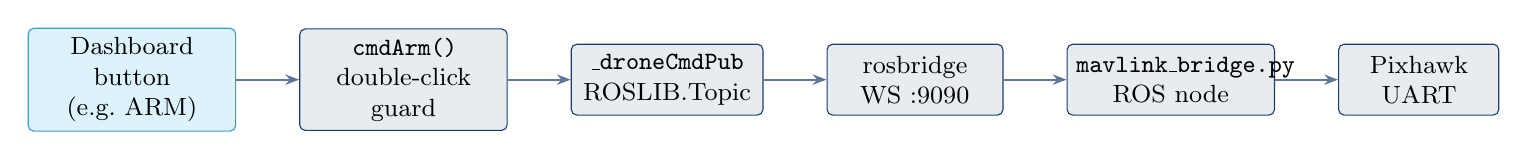
\begin{tikzpicture}[node distance=0.4cm and 0.9cm]
  \node[gcsblock, text width=2.4cm] (btn) {Dashboard button\\(e.g.\ ARM)};
  \node[block, text width=2.4cm, right=0.8cm of btn] (cmd) {\texttt{cmdArm()}\\double-click guard};
  \node[block, text width=2.2cm, right=0.8cm of cmd] (pub) {\texttt{\_droneCmdPub}\\ROSLIB.Topic};
  \node[block, text width=2.0cm, right=0.8cm of pub] (rb)  {rosbridge\\WS :9090};
  \node[block, text width=2.4cm, right=0.8cm of rb]  (bri) {\texttt{mavlink\_bridge.py}\\ROS node};
  \node[block, text width=1.8cm, right=0.8cm of bri] (px)  {Pixhawk\\UART};
  \draw[arrow] (btn) -- (cmd);
  \draw[arrow] (cmd) -- (pub);
  \draw[arrow] (pub) -- (rb);
  \draw[arrow] (rb)  -- (bri);
  \draw[arrow] (bri) -- (px);
\end{tikzpicture}%
}
\end{center}

The ARM command has an additional safety interlock: a first click sets a
timestamp; a second click within 800 ms confirms and sends the command.
A single click only shows ``click again to confirm'' in the command log.

\subsubsection{Service management}

The Services panel sends start/stop JSON to \texttt{/gcs/cmd}, which
\texttt{gcs\_control.py} receives and acts on. An additional auto-start
rule is applied in the frontend:

\begin{lstlisting}[style=javascript, caption=Auto-start cameras when barcode service starts]
if (svc === 'barcode' && action === 'start') {
  // Barcode detector needs a camera source -- ensure it is running
  ['camera', 'camera2', 'mjpeg'].forEach(s => {
    if (S.svcStatus[s] !== 'running') {
      _svcPub.publish(new ROSLIB.Message({
        data: JSON.stringify({ action: 'start', service: s })
      }))
    }
  })
}
\end{lstlisting}

% =============================================================================
\section{Complete ROS2 Topic Map}
% =============================================================================

{\footnotesize
\begin{longtable}{>{\ttfamily\raggedright\arraybackslash}p{4.8cm}
                  >{\raggedright\arraybackslash}p{2.4cm}
                  >{\raggedright\arraybackslash}p{3.0cm}
                  >{\raggedright\arraybackslash}p{3.4cm}}
  \toprule
  \normalfont\textbf{Topic} & \textbf{Publisher} & \textbf{Subscriber(s)} & \textbf{Content} \\
  \midrule
  /camera/forward/image\_raw/compressed & camera\_publisher & barcode\_detector, app.js & JPEG frames \\[2pt]
  /barcode/roi/image/compressed & barcode\_detector & app.js & Annotated JPEG \\[2pt]
  /barcode/detection & barcode\_detector & app.js & Detection JSON \\[2pt]
  /drone/vfr & mavlink\_bridge & app.js & Speed/alt/heading \\[2pt]
  /drone/state & mavlink\_bridge & app.js & Armed/mode/connected \\[2pt]
  /drone/motors & mavlink\_bridge & app.js & PWM channels \\[2pt]
  /drone/gps\_status & mavlink\_bridge & app.js & Fix/satellites \\[2pt]
  /drone/cmd & app.js & mavlink\_bridge & Flight commands \\[2pt]
  /mavros/battery & mavlink\_bridge & app.js & Voltage / \% \\[2pt]
  /mavros/imu/data & mavlink\_bridge & app.js & Quat. / ang. vel. \\[2pt]
  /mavros/global\_position/global & mavlink\_bridge & brain\_node, app.js & GPS NavSatFix \\[2pt]
  /mavros/local\_position/velocity\_body & mavlink\_bridge & app.js & NED velocities \\[2pt]
  /mavros/setpoint\_position/local & brain\_node & Pixhawk & Waypoint target \\[2pt]
  /brain/planned\_path & brain\_node & app.js & Mission JSON \\[2pt]
  /Odometry & Point-LIO & barcode\_detector, brain\_node & SLAM pose \\[2pt]
  /tf & Point-LIO & barcode\_detector & TF transforms \\[2pt]
  /gcs/cmd & app.js & gcs\_control & Start/stop services \\[2pt]
  /gcs/status & gcs\_control & app.js & Service states \\
  \bottomrule
\end{longtable}
}

% =============================================================================
\section{Deployment Quick Reference}
% =============================================================================

\subsection{Raspberry Pi prerequisites}

\begin{enumerate}
  \item Add \texttt{enable\_uart=1} to \texttt{/boot/firmware/config.txt} and reboot.
  \item Install Python dependencies:
  \begin{lstlisting}[style=bash]
pip3 install --break-system-packages pymavlink pyzbar opencv-python flask
  \end{lstlisting}
  \item Install systemd service:
  \begin{lstlisting}[style=bash]
sudo cp ~/rosbridge.service /etc/systemd/system/
sudo systemctl daemon-reload && sudo systemctl enable --now rosbridge
  \end{lstlisting}
\end{enumerate}

\subsection{Deploy updated files}

\begin{lstlisting}[style=bash, caption=SCP individual file to Pi]
scp mavlink_bridge.py raspi5@172.20.10.2:~/mavlink_bridge.py
\end{lstlisting}

\subsection{GCS app (laptop)}

\begin{lstlisting}[style=bash]
npm install       # first time only
npm start         # development
npm run build     # create installer (Win / Linux / macOS)
\end{lstlisting}

\subsection{Environment variables}

\begin{center}
\begin{tabular}{lll}
  \toprule
  \textbf{Variable} & \textbf{Default} & \textbf{Effect} \\
  \midrule
  \texttt{MAV\_PORT} & auto-detect & Override serial port \\
  \texttt{MAV\_BAUD} & 57600 & Override baud rate \\
  \texttt{ROS\_DISTRO} & jazzy & ROS2 distro name \\
  \bottomrule
\end{tabular}
\end{center}

\vfill
\noindent\textcolor{navyblue!40}{\rule{\textwidth}{0.4pt}}\\
{\small\color{gray}
Drone GCS — PAE-EDISA 2025--2026 · UPC ·
\href{https://github.com/clarajorba/PAE-EDISA-2026}{github.com/clarajorba/PAE-EDISA-2026}}

\end{document}
